\chapter{Archaea and Bacteria}\label{archaea-and-bacteria}

In biological
\href{https://en.wikipedia.org/wiki/Taxonomy_(biology)}{taxonomy}, a
domain is the highest taxonomic rank of organisms in the
\href{https://en.wikipedia.org/wiki/Three-domain_system}{three-domain
system} of taxonomy designed by Carl Woese, an American microbiologist
and biophysicist. According to the Woese system, introduced in 1990, the
tree of life consists of three domains: Archaea, Bacteria, and Eukarya.
The first two are all prokaryotic microorganisms, or single-celled
organisms whose cells have no nucleus. All life that has a nucleus and
membrane-bound organelles, and multicellular organisms, is included in
the Eukarya.

\section{Bacteria}\label{bacteria}

\href{https://en.wikipedia.org/wiki/Bacteria}{Bacteria} (singular:
bacterium) are prokaryotic microorganisms. Typically, a few micrometers
in length, bacteria have a number of shapes, ranging from spheres to
rods and spirals. Bacteria were among the first life forms to appear on
Earth, and are present in most of its habitats. Bacteria inhabit soil,
water, acidic hot springs, radioactive waste, and the deep portions of
Earth's crust. Bacteria also live in symbiotic and parasitic
relationships with plants and animals. Most bacteria have not been
characterized, and only about half of the bacterial phyla have species
that can be grown in the laboratory. The study of bacteria is known as
bacteriology, a branch of microbiology. There are typically 40 million
bacterial cells in a gram of soil and a million bacterial cells in a
milliliter of fresh water. There are approximately
5x10\textsuperscript{30} bacteria on Earth forming a biomass which
exceeds that of all plants and animals. Bacteria are vital in many
stages of the nutrient cycle by recycling nutrients such as the fixation
of nitrogen from the atmosphere. The nutrient cycle includes the
decomposition of dead bodies and bacteria are responsible for the
putrefaction stage in this process. In the biological communities
surrounding hydrothermal vents and cold seeps, extremophile bacteria
provide the nutrients needed to sustain life by converting dissolved
compounds, such as hydrogen sulfide and methane, to energy. In March
2013, data reported by researchers in October 2012, was published. It
was suggested that bacteria thrive in the Mariana Trench, which with a
depth of up to 11 kilometers is the deepest known part of the oceans.
Other researchers reported related studies that microbes thrive inside
rocks up to 580 meters below the sea floor under 2.6 kilometers of ocean
off the coast of the northwestern United States. The largest number of
bacteria in humans exist in the gut flora, and a large number on the
skin. The vast majority of the bacteria in the body are rendered
harmless by the protective effects of the immune system, though many are
beneficial particularly in the gut flora. However, several species of
bacteria are pathogenic and cause infectious diseases. The most common
fatal bacterial diseases are respiratory infections, with tuberculosis
alone killing about 2 million people per year, mostly in sub-Saharan
Africa. In developed countries, antibiotics are used to treat bacterial
infections and are also used in farming, making antibiotic resistance a
growing problem. In industry, bacteria are important in sewage treatment
and the breakdown of oil spills, the production of cheese and yogurt
through fermentation, and the recovery of gold, palladium, copper and
other metals in the mining sector, as well as in biotechnology, and the
manufacture of antibiotics and other chemicals.

\section{Archaea}\label{archaea}

\href{https://en.wikipedia.org/wiki/Archaea}{Archaea} have unique
properties separating them from the other two domains of life, Bacteria
and Eukaryota. The Archaea are further divided into multiple recognized
phyla. Classification is difficult because the majority have not been
isolated in the laboratory and have only been detected by analysis of
their nucleic acids in samples from their environment. Archaea and
bacteria are generally similar in size and shape, although a few archaea
have very strange shapes. Despite this morphological similarity to
bacteria, archaea possess genes and several metabolic pathways that are
more closely related to those of eukaryotes, notably the enzymes
involved in transcription and translation. Other aspects of archaeal
biochemistry are unique, such as their reliance on ether lipids in their
cell membranes. Archaea use more energy sources than eukaryotes: these
range from organic compounds, such as sugars, to ammonia, metal ions or
even hydrogen gas. Salt-tolerant archaea use sunlight as an energy
source, and other species of archaea fix carbon; however, unlike plants
and cyanobacteria, no known species of archaea does both. Archaea
reproduce asexually by binary fission, fragmentation, or budding; unlike
bacteria and eukaryotes, no known species forms spores. Archaea were
initially viewed as extremophiles living in harsh environments, such as
hot springs and salt lakes, but they have since been found in a broad
range of habitats, including soils, oceans, and marshlands. They are
also part of the human microbiota, found in the colon, oral cavity, and
skin. Archaea are particularly numerous in the oceans, and the archaea
in plankton may be one of the most abundant groups of organisms on the
planet. Archaea are a major part of Earth's life and may play roles in
both the carbon cycle and the nitrogen cycle. No clear examples of
archaeal pathogens or parasites are known, but they are often mutualists
or commensals. One example is the methanogens that inhabit human and
ruminant guts, where their vast numbers aid digestion. Methanogens are
also used in biogas production and sewage treatment, and biotechnology
exploits enzymes from extremophile archaea that can endure high
temperatures and organic solvents.

\section{Eukarya}\label{eukarya}

Members of the domain Eukarya are called
\href{https://en.wikipedia.org/wiki/Eukaryote}{eukaryotes}. A eukaryote
is any organism whose cells have a cell nucleus and other organelles
enclosed within membranes) can be unicellular or multicellular
organisms. The defining feature that sets eukaryotic cells apart from
prokaryotic cells (Bacteria and Archaea) is that they have
membrane-bound organelles, especially the nucleus, which contains the
genetic material enclosed by the nuclear membrane. The presence of a
nucleus gives eukaryotes their name, which comes from the Greek eu,
``well'' or ``true'' and karyon, ``nut'' or ``kernel''. Eukaryotic cells
also contain other membrane-bound organelles such as mitochondria,
endoplasmic reticulum and the Golgi apparatus. In addition, plants and
algae contain chloroplasts. Unlike unicellular archaea and bacteria,
eukaryotes may also be multicellular and include organisms consisting of
many kinds of tissue and cell types. Eukaryotes can reproduce both
asexually through mitosis and sexually through meiosis and gamete
fusion. In mitosis, one cell divides to produce two genetically
identical cells. In meiosis, DNA replication is followed by two rounds
of cell division to produce four haploid daughter cells. These act as
sex cells (gametes). Each gamete has just one set of chromosomes, each a
unique mix of the corresponding pair of parental chromosomes resulting
from genetic recombination during meiosis. Eukaryotes evolved
approximately 1.6-2.1 billion years ago, during the Proterozoic eon.

\href{https://en.wikipedia.org/wiki/Virus}{Viruses} are not part of the
three-domain system.

\section{Gram stain}\label{gram-stain}

\href{https://en.wikipedia.org/wiki/Gram_stain}{Gram stain} or Gram
staining (Figure \ref{fig:gram}), also called Gram's method, is a method
of staining used to distinguish and classify bacterial species into two
large groups (gram-positive and gram-negative). The name comes from the
Danish bacteriologist Hans Christian Gram, who developed the technique.

\begin{figure}

{\centering 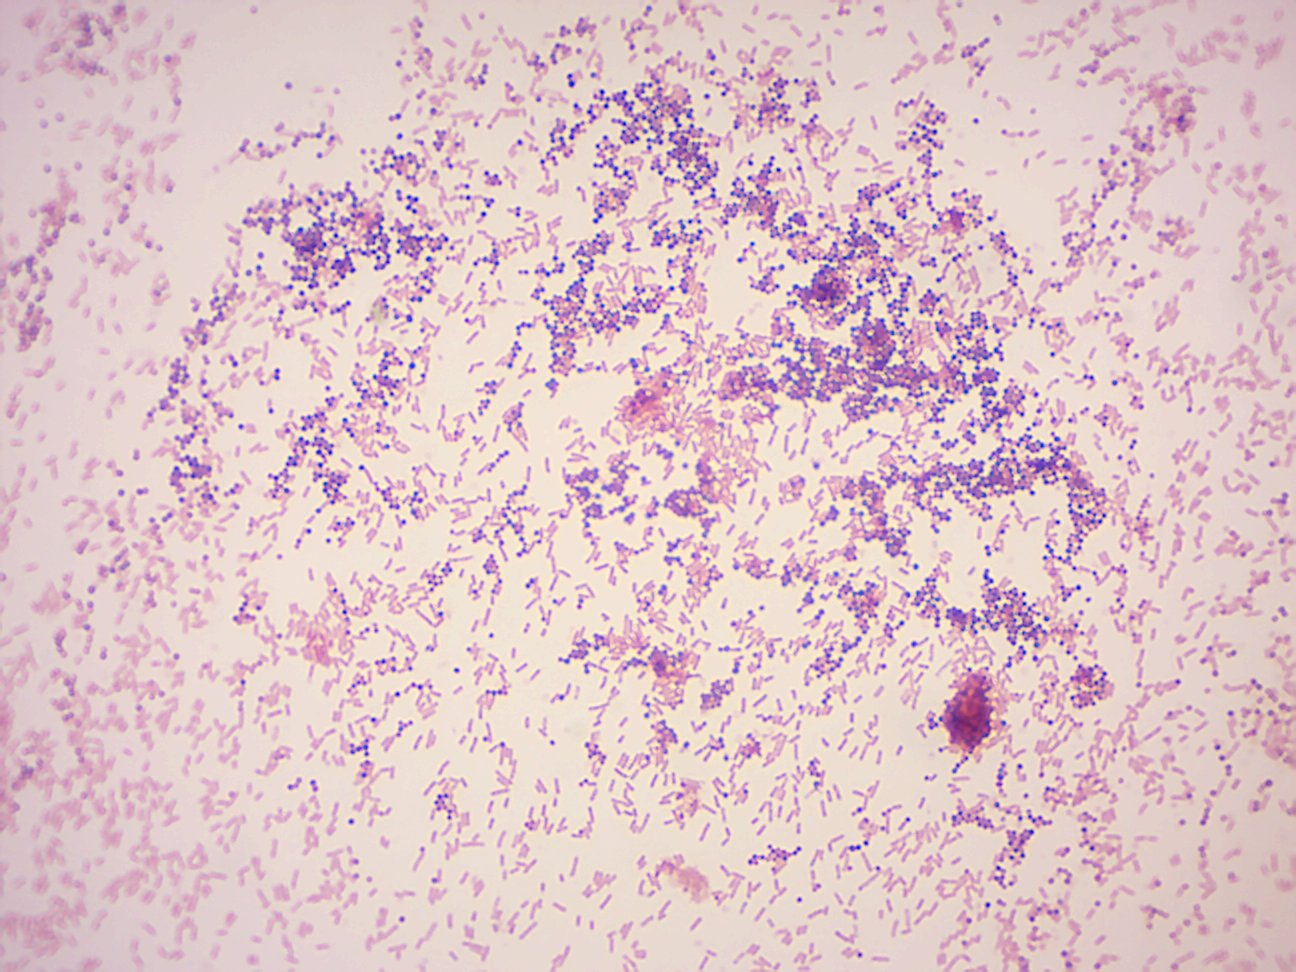
\includegraphics[width=0.7\linewidth]{./figures/bacteria/Gram_stain} 

}

\caption{Gram stained bacteria.}\label{fig:gram}
\end{figure}

Gram staining differentiates bacteria by the chemical and physical
properties of their cell walls by detecting peptidoglycan, which is
present in the cell wall of Gram-positive bacteria. Gram-negative cells
also contain peptidoglycan, but a very small layer of it that is
dissolved when the alcohol is added. This is why the cell loses its
initial color from the primary stain. Gram-positive bacteria retain the
crystal violet dye, and thus are stained violet, while the Gram-negative
bacteria do not; after washing, a counterstain is added (safranin) that
will stain these Gram-negative bacteria a pink color. Both Gram-positive
bacteria and Gram-negative bacteria pick up the counterstain. The
counterstain, however, is unseen on Gram-positive bacteria because of
the darker crystal violet stain.

\subsection{Experimental procedures}\label{experimental-procedures-35}

\begin{enumerate}
\def\labelenumi{\arabic{enumi}.}
\tightlist
\item
  Use a bacterial loop to pick up bacteria (Staphylococcus aureus and
  Escherichia coli) from the culture plate and streak out on a slide so
  that both samples partially overlap in the middle of the slide. Heat
  fix the sample to the slide by carefully passing the slide three times
  through a Bunsen burner flame.
\item
  Add crystal violet to the slide and incubate for 1 minute. Rinse slide
  with a gentle stream of water to remove unbound crystal violet.
\item
  Add Gram's iodine for 1 minute- this is the mordant, an agent that
  fixes the crystal violet to the bacterial cell wall.
\item
  Rinse slide with decolorizer until no more dye is running off. Rinse
  with a gentle stream of water.
\item
  Add safranin to the slide and incubate for 1 minute. Wash with a
  gentle stream of water. Gram positive bacteria it will retain crystal
  violet and stain purple. Gram negative will lose the primary stain and
  take the secondary stain causing it to appear pink when viewed under a
  microscope.
\item
  View under the microscope.
\end{enumerate}

\section{View living organisms}\label{view-living-organisms}

\subsection{Oscillatoria}\label{oscillatoria}

\href{https://en.wikipedia.org/wiki/Oscillatoria}{\emph{Oscillatoria}}
is a genus of filamentous cyanobacterium which is named after the
oscillation in its movement (Figure \ref{fig:oscillatoria}). Filaments
in the colonies can slide back and forth against each other until the
whole mass is reoriented to its light source. It is commonly found in
watering-troughs waters, and is mainly blue-green or brown-green.
Oscillatoria is an organism that reproduces by fragmentation.
Oscillatoria forms long filaments of cells which can break into
fragments called hormogonia. The hormogonia can grow into a new, longer
filament. Breaks in the filament usually occur where dead cells
(necridia) are present. Oscillatoria uses photosynthesis to survive and
reproduce. Each filament of oscillatoria consists of trichome which is
made up of rows of cells. The tip of the trichome oscillates like a
pendulum.

\begin{figure}

{\centering 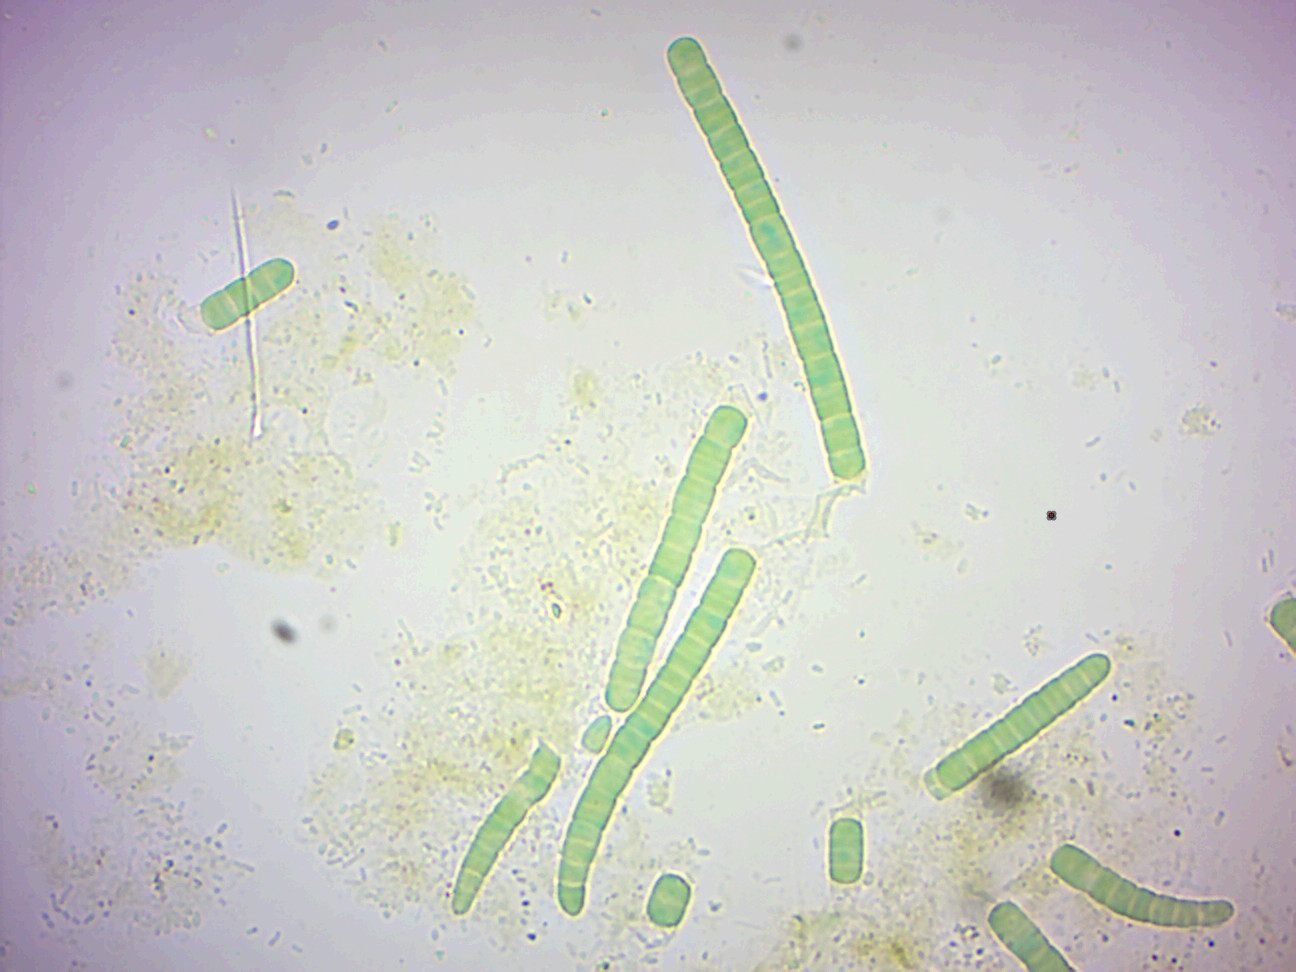
\includegraphics[width=0.7\linewidth]{./figures/bacteria/oscillatoria} 

}

\caption{Oscillatoria.}\label{fig:oscillatoria}
\end{figure}

\subsection{Nostoc}\label{nostoc}

\href{https://en.wikipedia.org/wiki/Nostoc}{\emph{Nostoc}} is a genus of
cyanobacteria found in various environments that forms colonies composed
of filaments of moniliform cells in a gelatinous sheath (Figure
\ref{fig:nostoc}). Nostoc can be found in soil, on moist rocks, at the
bottom of lakes and springs (both fresh- and saltwater), and rarely in
marine habitats. It may also grow symbiotically within the tissues of
plants, such as the evolutionarily ancient angiosperm Gunnera and the
hornworts (a group of bryophytes), providing nitrogen to its host
through the action of terminally differentiated cells known as
heterocysts. These bacteria contain photosynthetic pigments in their
cytoplasm to perform photosynthesis.

\begin{figure}

{\centering 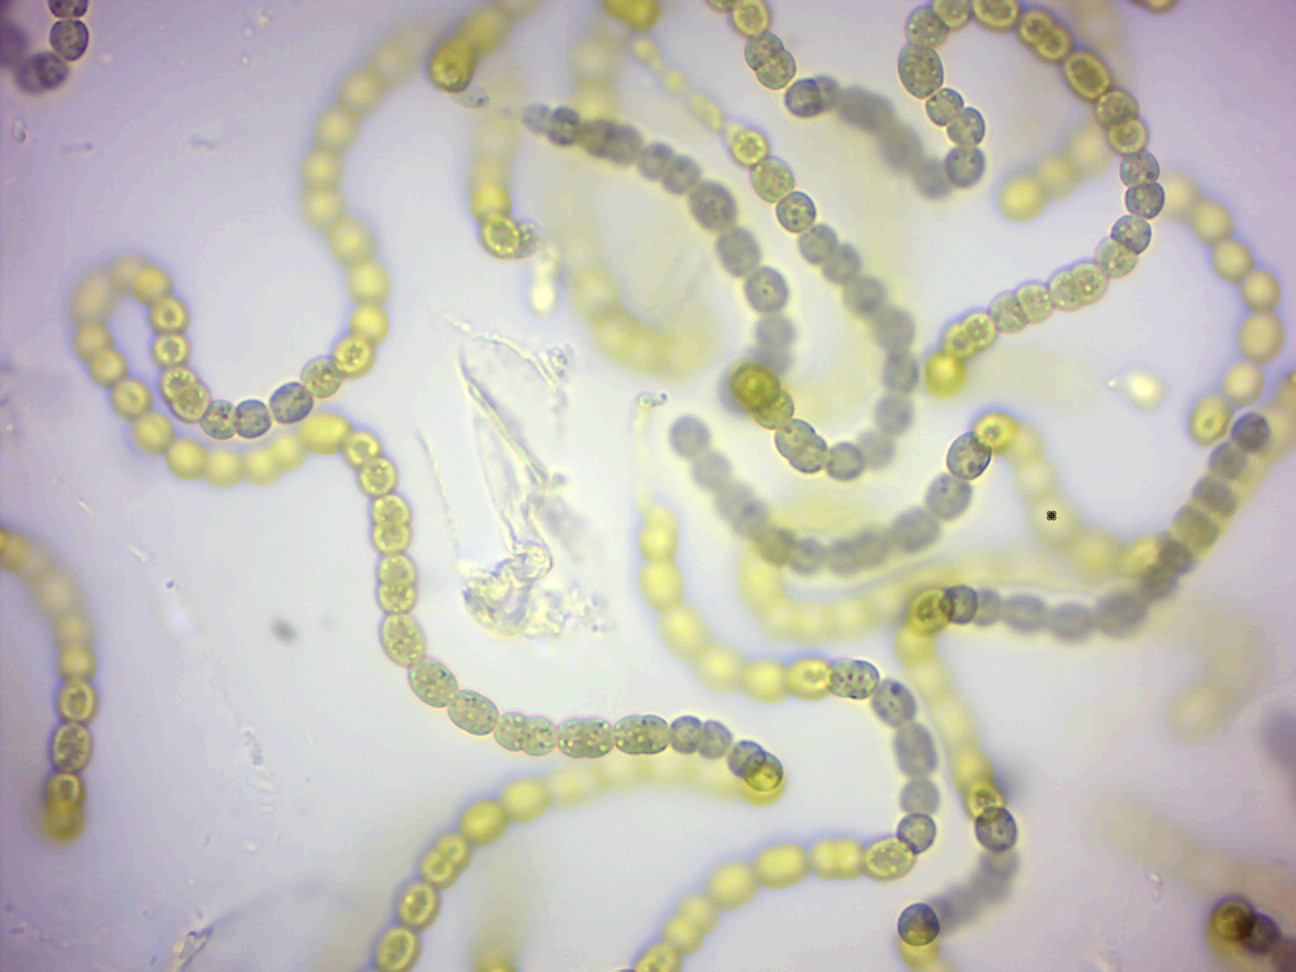
\includegraphics[width=0.7\linewidth]{./figures/bacteria/nostoc_live} 

}

\caption{Nostoc.}\label{fig:livenostoc}
\end{figure}

\subsection{Gloeocapsa}\label{gloeocapsa}

\href{https://en.wikipedia.org/wiki/Gloeocapsa}{\emph{Gloeocapsa}} (from
the Greek gloia (gelatinous) and the Latin capsa (case) is a genus of
cyanobacteria (Figure \ref{fig:gloeocapsa}). The cells secrete
individual gelatinous sheaths which can often be seen as sheaths around
recently divided cells within outer sheaths. Recently divided cell pairs
often appear to be only one cell since the new cells cohere temporarily.
They are also known as glow caps, a term derived from the yellowish hue
given off by the cap.

\begin{figure}

{\centering 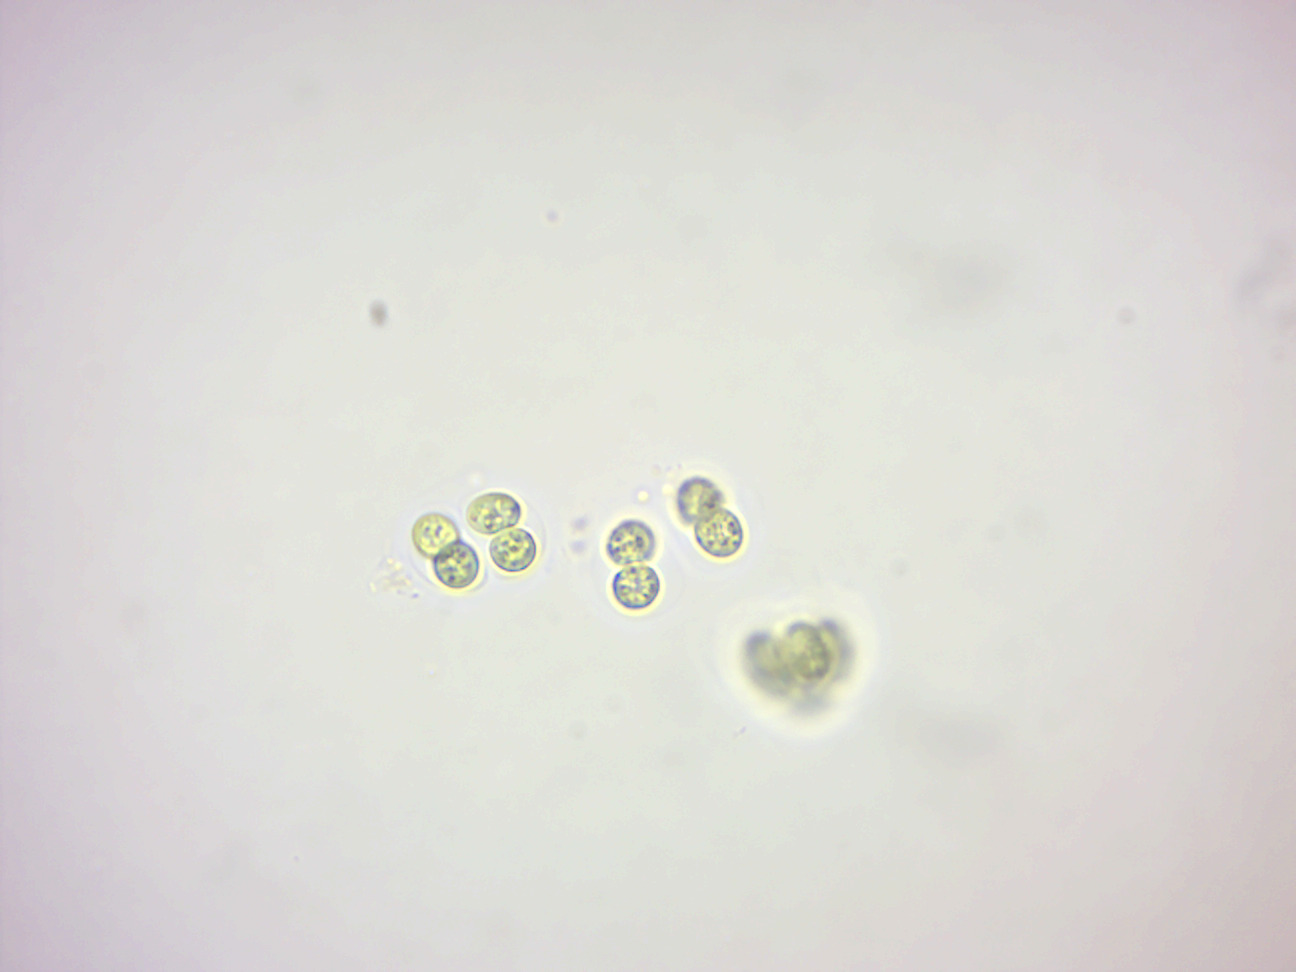
\includegraphics[width=0.7\linewidth]{./figures/bacteria/gloeocapsa} 

}

\caption{Gloeocapsa.}\label{fig:gloeocapsa}
\end{figure}

\section{View Prepared Slides}\label{view-prepared-slides-2}

\subsection{Mixed coccus (Gram stain) (Figure
\ref{fig:cocci})}\label{mixed-coccus-gram-stain-figure-reffigcocci}

\begin{figure}

{\centering 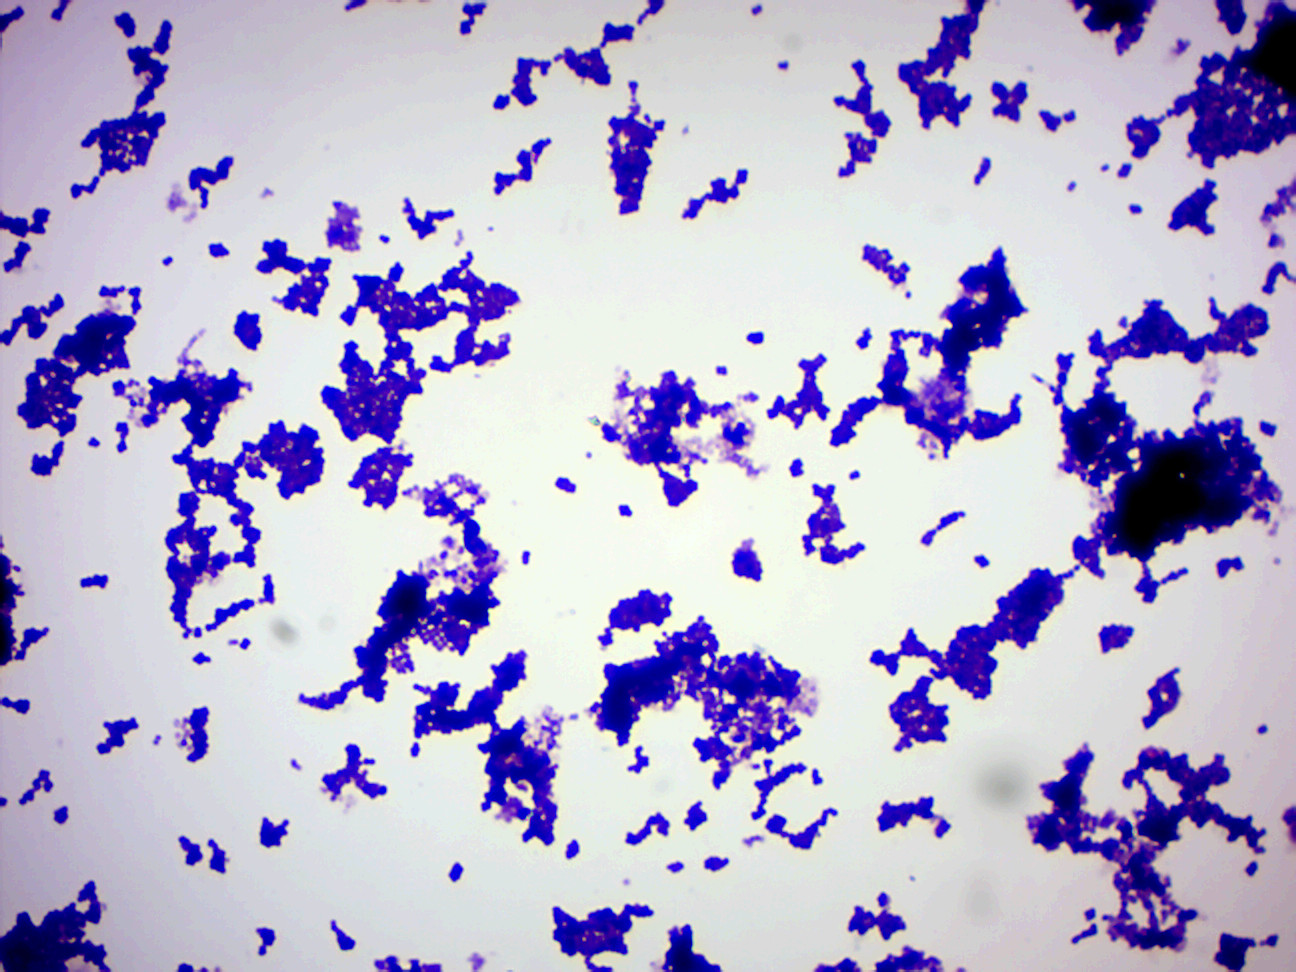
\includegraphics[width=0.7\linewidth]{./figures/bacteria/cocci} 

}

\caption{Mixed cocci.}\label{fig:cocci}
\end{figure}

\subsection{Mixed bacillus (Gram stain) (Figure
\ref{fig:bacilli})}\label{mixed-bacillus-gram-stain-figure-reffigbacilli}

\begin{figure}

{\centering 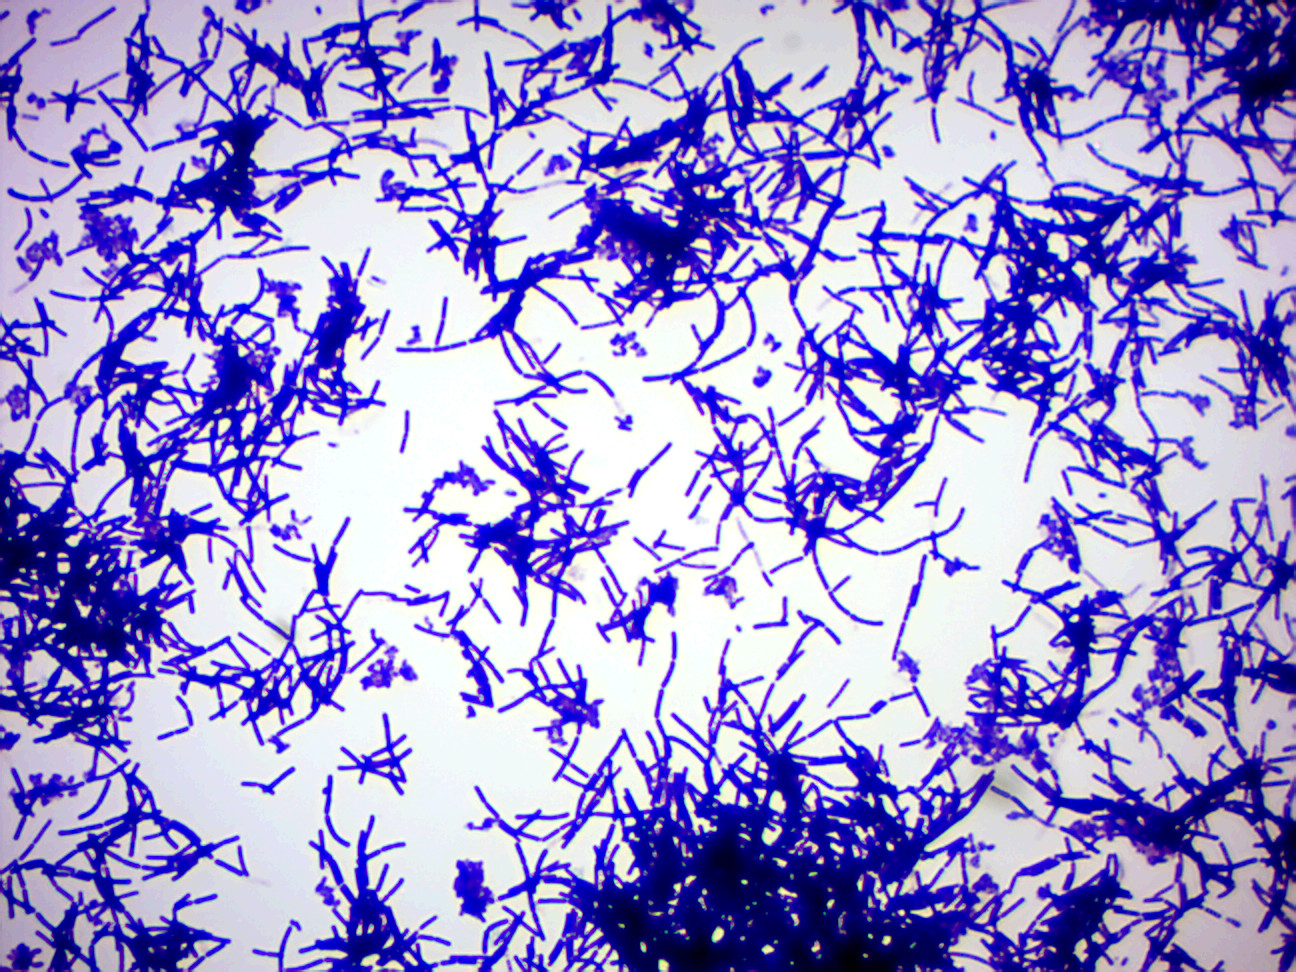
\includegraphics[width=0.7\linewidth]{./figures/bacteria/bacilli} 

}

\caption{Mixed bacilli.}\label{fig:bacilli}
\end{figure}

\subsection{Spirillum}\label{spirillum}

\href{https://en.wikipedia.org/wiki/Spirillum}{\emph{Spirillum}} is a
genus of Gram-negative bacteria (Figure \ref{fig:spirilla}). Members of
the genus Spirillum are large, elongate, spiral shaped, rigid cells.
Some have tufts of amphitrichous flagella at both poles. They are
microaerophilic and usually found in stagnant freshwater rich in organic
matter.

\begin{figure}

{\centering 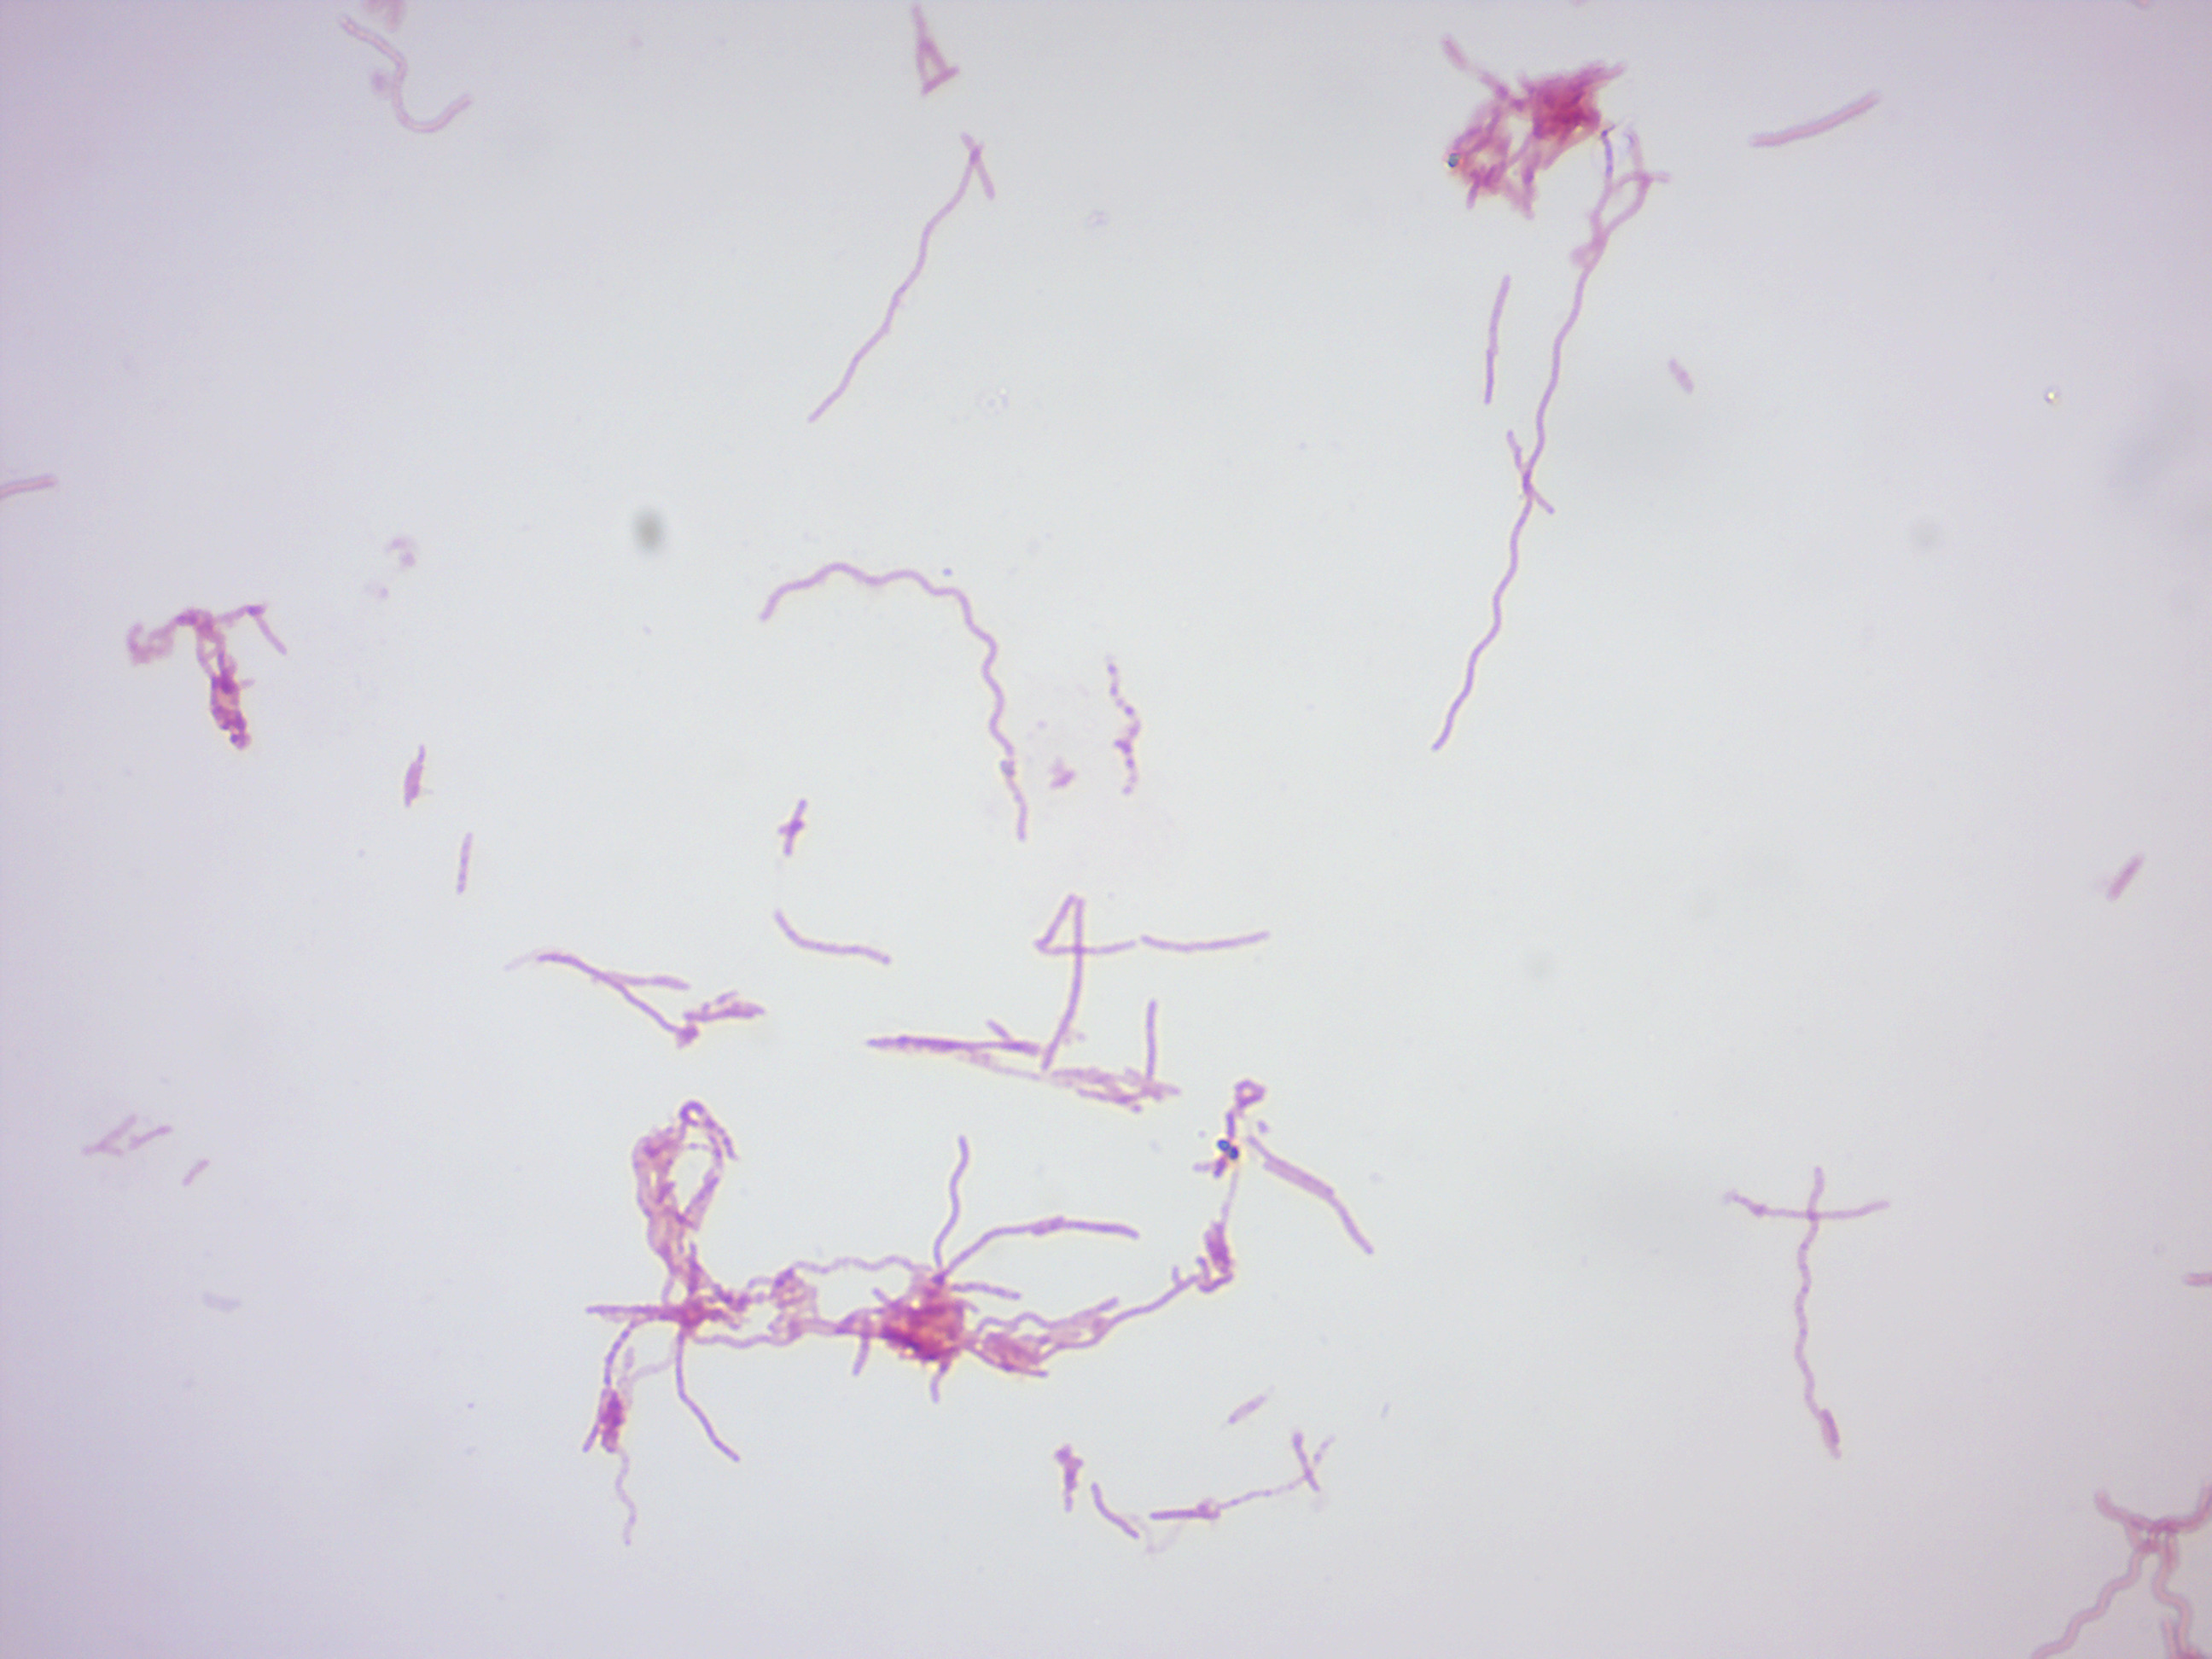
\includegraphics[width=0.7\linewidth]{./figures/bacteria/spirilla} 

}

\caption{Spirilla.}\label{fig:spirilla}
\end{figure}

\subsection{Treponema}\label{treponema}

\href{https://en.wikipedia.org/wiki/Treponema}{\emph{Treponema}} is a
genus of spiral-shaped Gram-negative bacteria (Figure
\ref{fig:treponema}). The major treponeme species of human pathogens is
Treponema pallidum, whose subspecies are responsible for diseases such
as syphilis, bejel, and yaws.

\begin{figure}

{\centering 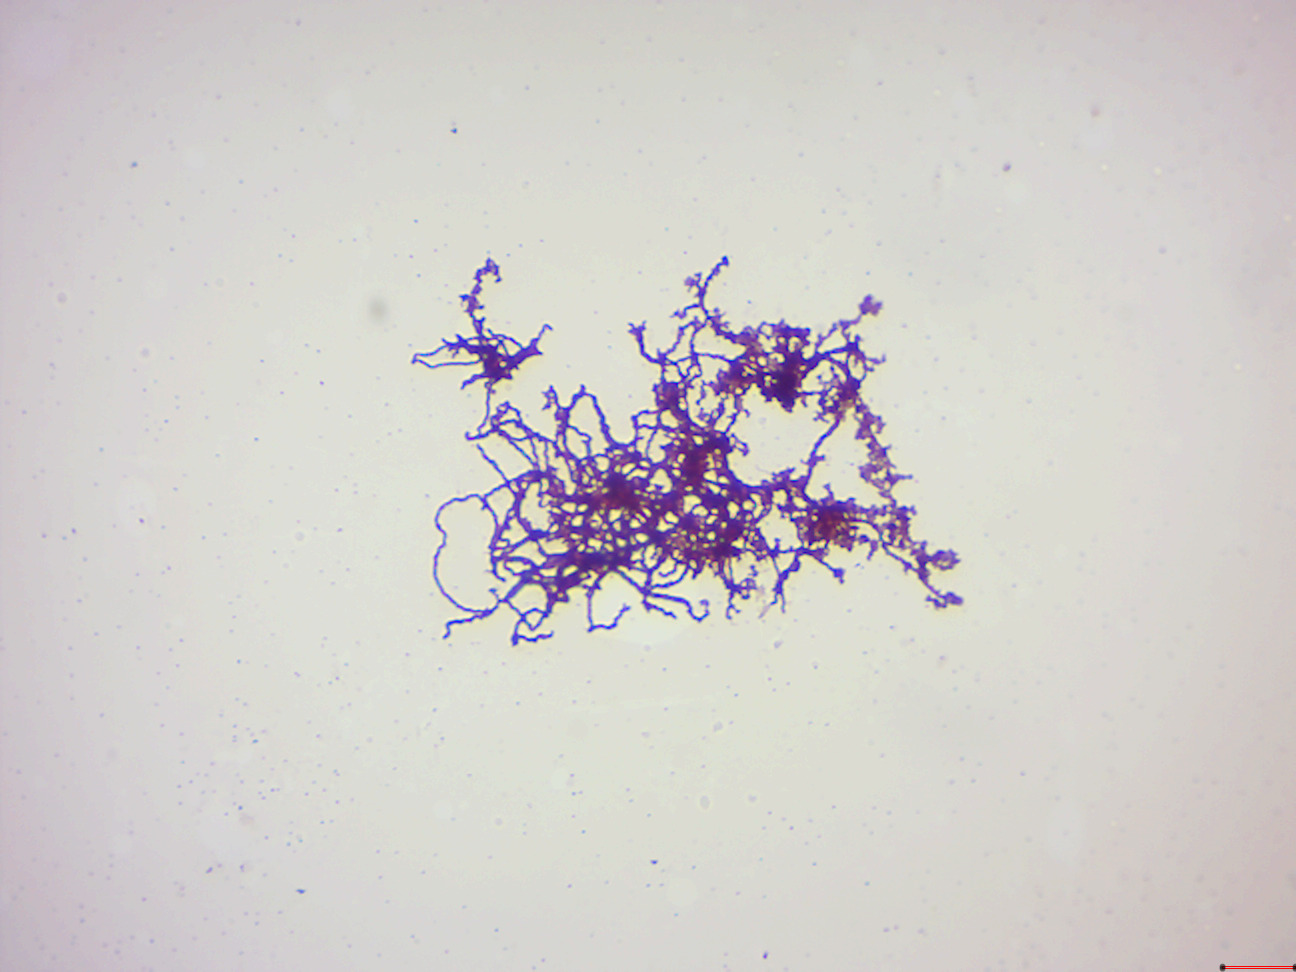
\includegraphics[width=0.7\linewidth]{./figures/bacteria/treponema} 

}

\caption{Treponema.}\label{fig:treponema}
\end{figure}

\subsection{Clostridium botulinum}\label{clostridium-botulinum}

\href{https://en.wikipedia.org/wiki/Clostridium_botulinum}{\emph{Clostridium
botulinum}} is a Gram-positive, rod-shaped, anaerobic, spore-forming,
motile bacterium with the ability to produce a neurotoxin known as
botulinum toxin. The botulinum toxin can cause a severe flaccid
paralytic disease in humans and other animals and is the most potent
toxin known to humankind, natural or synthetic, with a lethal dose of
1.3-2.1 ng/kg in humans. \emph{C. botulinum} is an obligate anaerobe,
meaning that oxygen is poisonous to the cells. However, it tolerates
traces of oxygen due to the enzyme superoxide dismutase, which is an
important antioxidant defense in nearly all cells exposed to oxygen. C.
botulinum is only able to produce the neurotoxin during sporulation,
which can only happen in an anaerobic environment. Other bacterial
species produce spores in an unfavorable growth environment to preserve
the organism's viability and permit survival in a dormant state until
the spores are exposed to favorable conditions.

\subsection{Staphylococcus aureus}\label{staphylococcus-aureus}

\href{https://en.wikipedia.org/wiki/Staphylococcus_aureus}{\emph{Staphylococcus
aureus}} (Figure \ref{fig:staph}) is a gram-positive, round-shaped
bacterium that is a member of the Firmicutes, and it is a member of the
normal flora of the body, frequently found in the nose, respiratory
tract, and on the skin. It is often positive for catalase and nitrate
reduction and is a facultative anaerobe that can grow without the need
for oxygen. Although S. aureus is not always pathogenic (and can
commonly be found existing as a commensal), it is a common cause of skin
infections including abscesses, respiratory infections such as
sinusitis, and food poisoning. Pathogenic strains often promote
infections by producing virulence factors such as potent protein toxins,
and the expression of a cell-surface protein that binds and inactivates
antibodies. The emergence of antibiotic-resistant strains of S. aureus
such as methicillin-resistant S. aureus (MRSA) is a worldwide problem in
clinical medicine.

\begin{figure}

{\centering 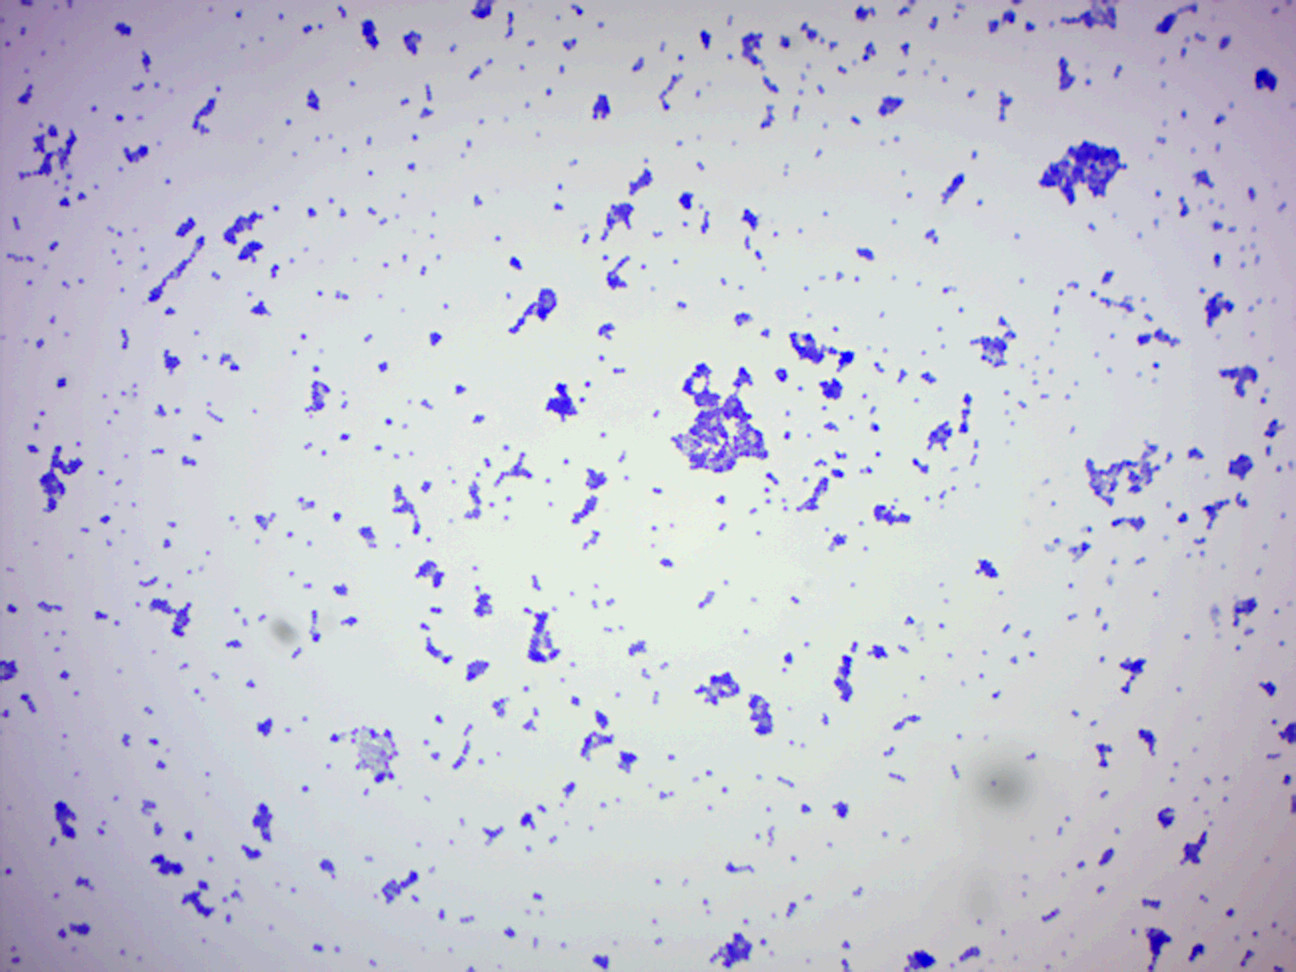
\includegraphics[width=0.7\linewidth]{./figures/bacteria/staphaureus} 

}

\caption{Staphylococcus aureus.}\label{fig:staph}
\end{figure}

\subsection{Oscillatoria}\label{oscillatoria-1}

\subsection{Nostoc (Figure
\ref{fig:nostoc})}\label{nostoc-figure-reffignostoc}

\begin{figure}

{\centering 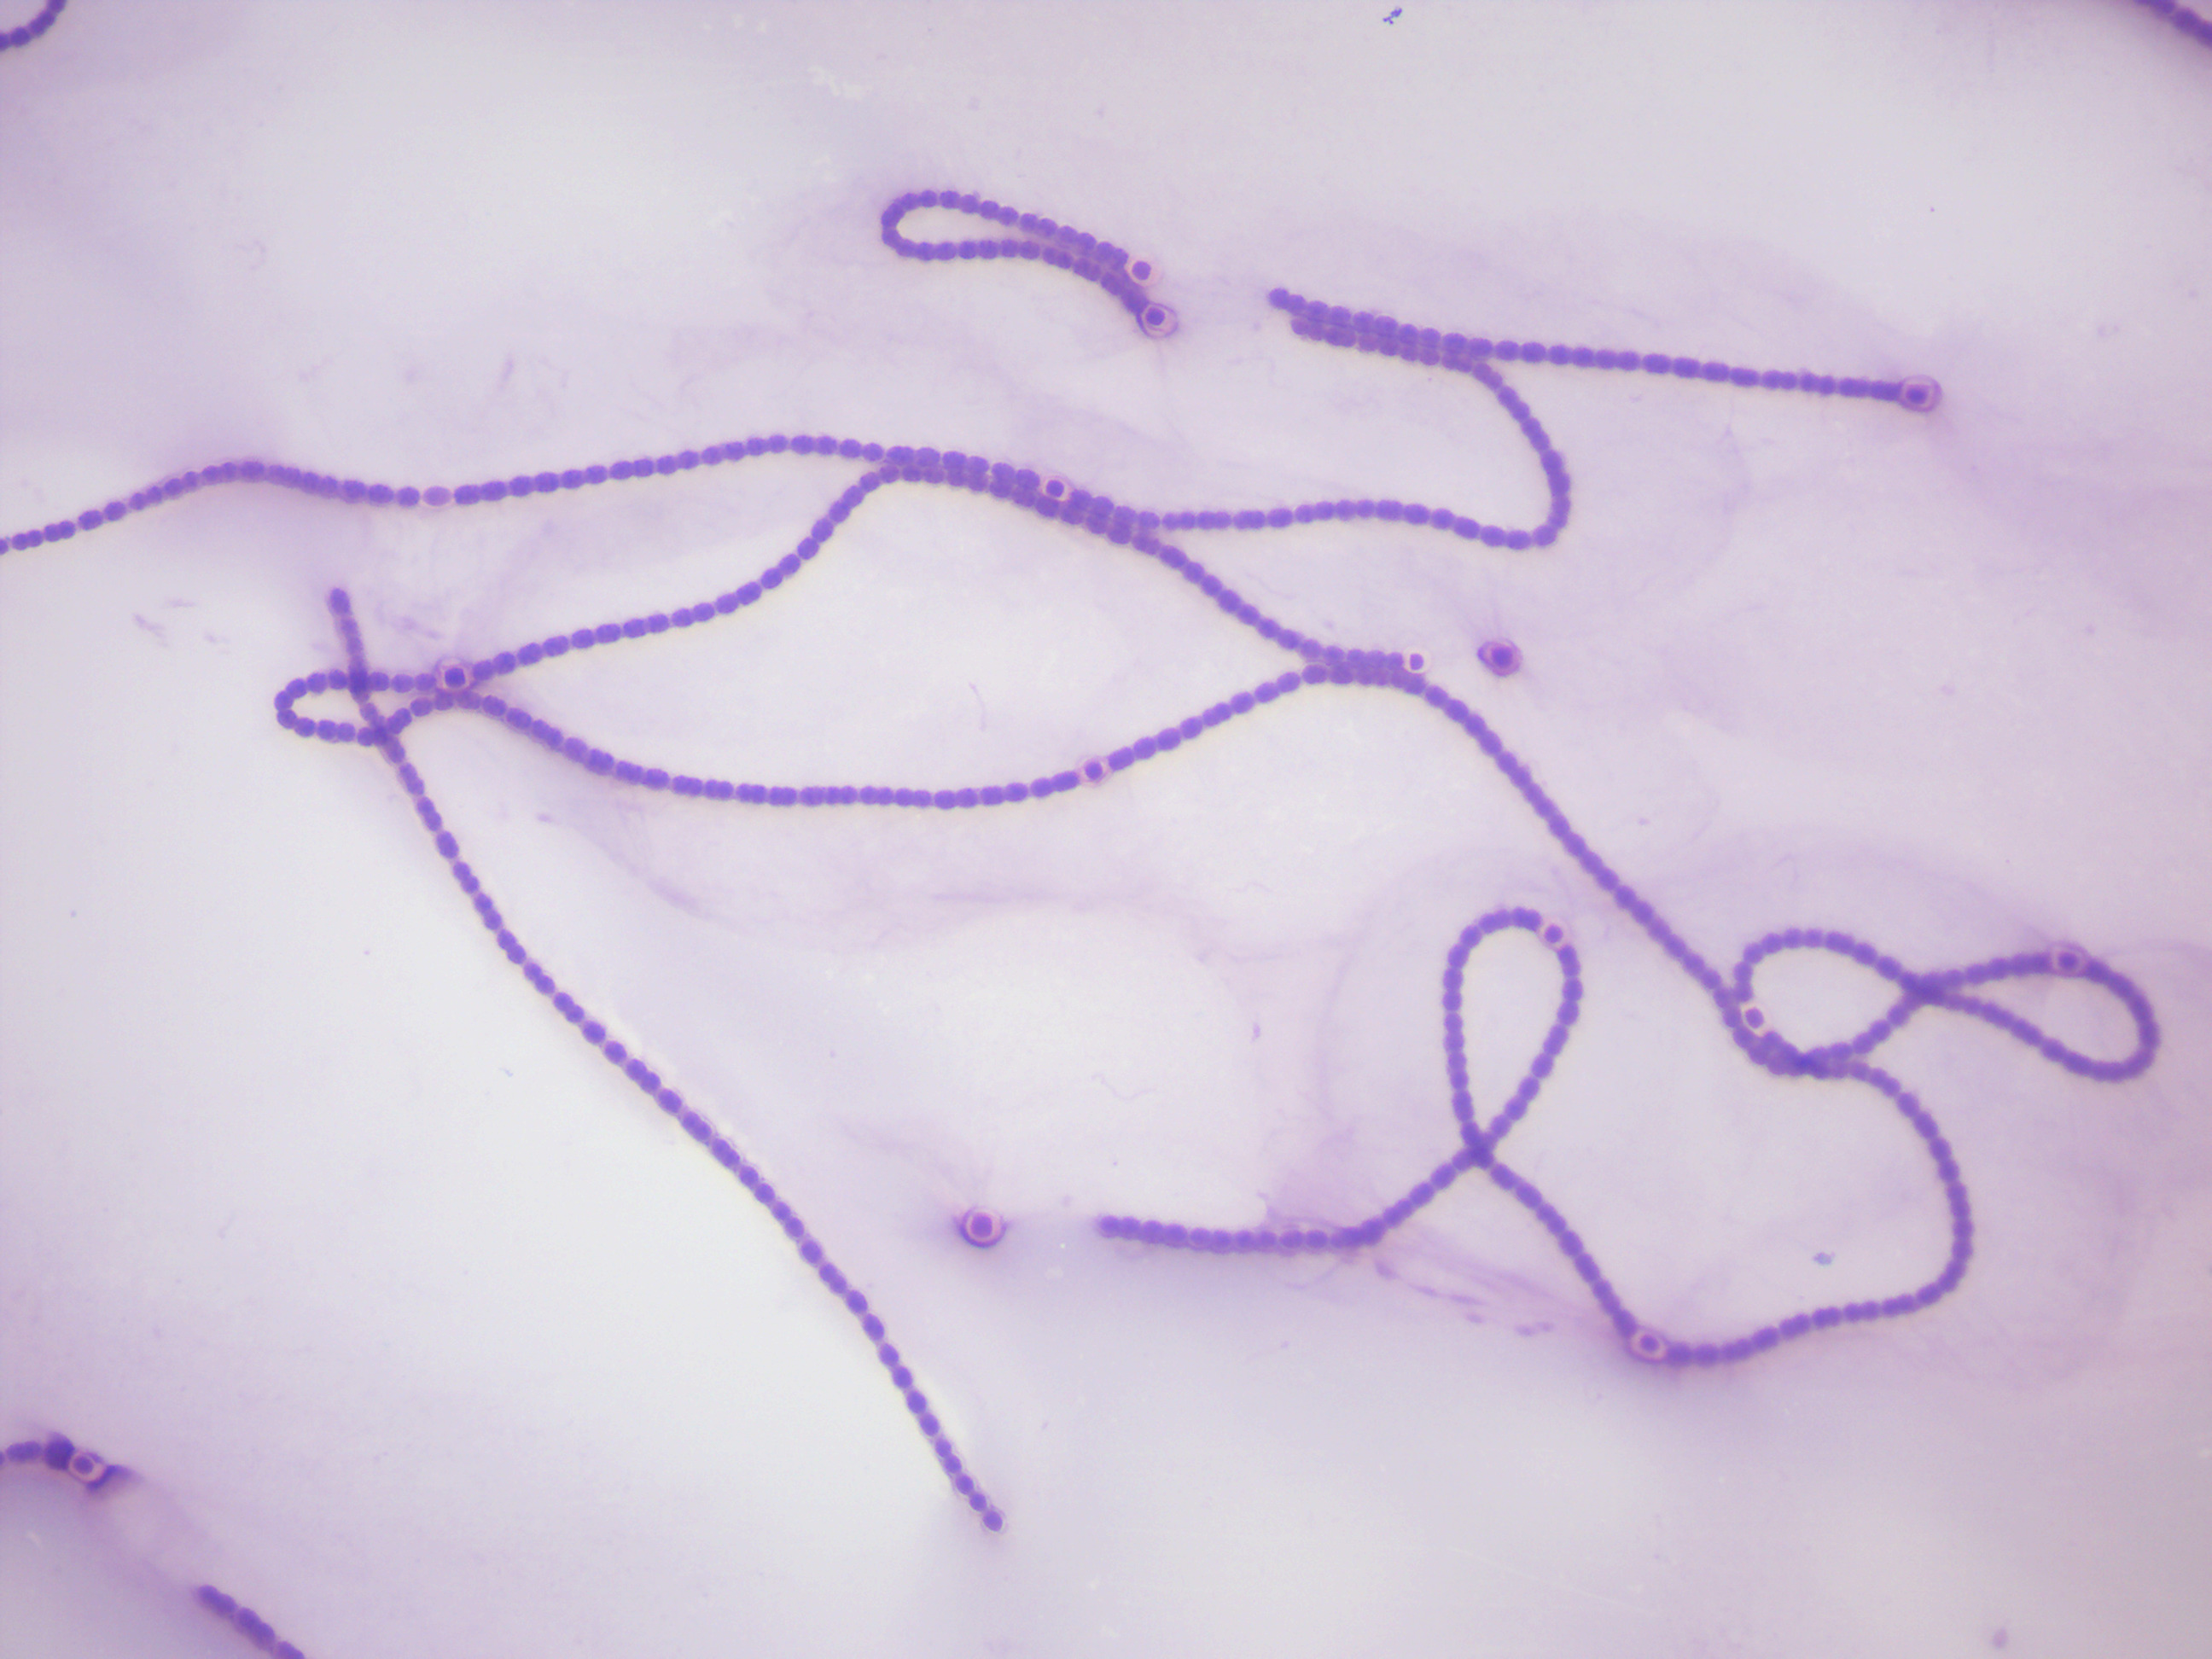
\includegraphics[width=0.7\linewidth]{./figures/bacteria/nostoc} 

}

\caption{Nostoc.}\label{fig:nostoc}
\end{figure}

\subsection{Anabaena}\label{anabaena}

\href{https://en.wikipedia.org/wiki/Anabaena}{\emph{Anabaena}} is a
genus of filamentous cyanobacteria that exist as plankton (Figure
\ref{fig:anabaena}). They are known for nitrogen-fixing abilities, and
they form symbiotic relationships with certain plants, such as the
mosquito fern. They are one of four genera of cyanobacteria that produce
neurotoxins, which are harmful to local wildlife, as well as farm
animals and pets. Production of these neurotoxins is assumed to be an
input into its symbiotic relationships, protecting the plant from
grazing pressure.

\begin{figure}

{\centering 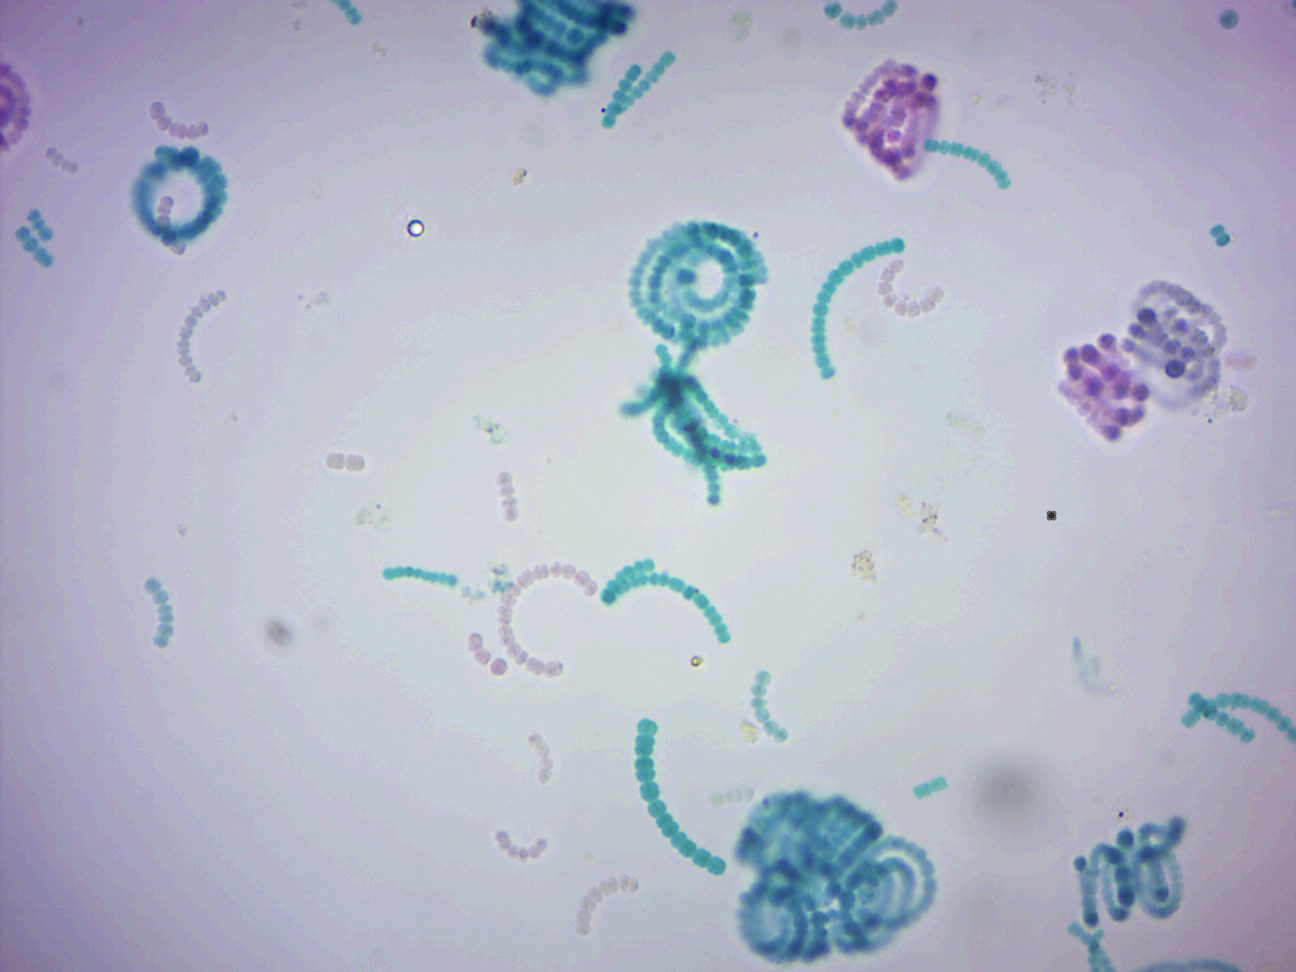
\includegraphics[width=0.7\linewidth]{./figures/bacteria/anabaena} 

}

\caption{Anabaena.}\label{fig:anabaena}
\end{figure}

\section{Review Questions}\label{review-questions-9}

\begin{enumerate}
\def\labelenumi{\arabic{enumi}.}
\tightlist
\item
  What are bacteria?
\item
  What are archaea?
\item
  What are eukarya?
\item
  What are cyanobacteria?
\end{enumerate}
